\documentclass[11pt,a4paper]{article}
\usepackage[utf8]{inputenc}
\usepackage{ngerman}
\usepackage{amsmath}
\usepackage{amsfonts}
\usepackage{amssymb}
\usepackage{graphicx}
\usepackage{tikz}
\usetikzlibrary{arrows, automata, positioning}
\begin{document}
	\title{Übung Nr.1 zur Vorlesung IPI}
	\author{David Bubeck und Patrick Nisble}
	\maketitle
	\section{''Fahrkartenautomat''}
		\begin{figure}[h]
			\centering
			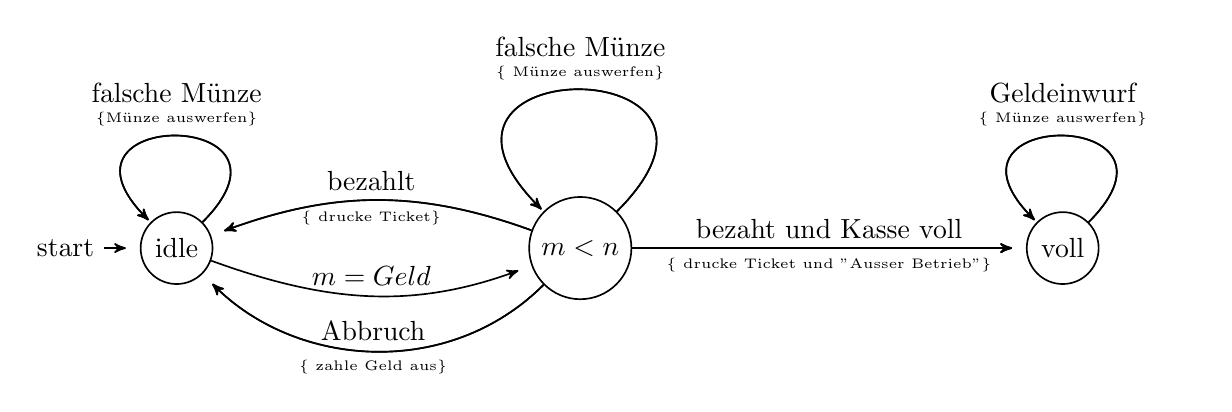
\begin{tikzpicture}[->, >=stealth', shorten >=5pt, semithick]
			
				\node [initial, state] 		(1)					{idle};
				\node [state]				(2)	[right = 4cm of 1]	{$m<n$};
				\node [state]				(3) [right = 5cm of 2]	{voll};
				
				\path	(1)	edge [loop, above] 				node[above=.3cm] {falsche Münze} 			(1)
							edge [loop, above]				node[above] {\tiny \{Münze auswerfen\}} (2)
				
							edge [in=200, out=340, above] 	node {$m = Geld$} 				(2)
				
						(2) edge [loop, above] 				node[above=.3cm] {falsche Münze}(2)
							edge [loop, above]				node[above] {\tiny \{ Münze auswerfen\} } 		(2)
				
							edge [out=225, in=315, above] 	node {Abbruch} 				(1)
							edge [out=225, in=315, below]	node {\tiny \{ zahle Geld aus\}}	(1)
				
							edge [in=20, out=160, above] 	node {bezahlt} 				(1) 
							edge [in=20, out=160, below]	node {\tiny \{ drucke Ticket\}} 	(1)
							
							edge [above]					node {bezaht und Kasse voll}(3)
							edge [below]					node {\tiny \{ drucke Ticket und ''Ausser Betrieb''\}} (3)
							
						(3)	edge [loop, above]				node[above=.3cm] {Geldeinwurf}	(3)
							edge [loop, above]				node[above] {\tiny \{ Münze auswerfen\}} (3)
				;
			
			\end{tikzpicture}
			
			\caption{Fahrkartenautomat, m: Momentanbetrag, n = Sollbetrag}
			\label{fig:f1}
		\end{figure}
		
	\section{Automat: ''Bibliothek''}
		\begin{figure}[h]
			\centering
			
			\begin{tabular}{c | p{2.5cm} p{2.5cm} p{2.5cm} p{4cm}}
				&	neues Buch	&	Buch abgeben	&	Buch ausleihen 	&	Ausleihfrist abgelaufen	\\ \hline
									
				Grundzustand	&	\tiny Buch wird katalogisiert und ist ausleihbar	& - &	\tiny ''Buch nicht verfügbar''	& -	\\
				
				
			\end{tabular}
			
			\caption{Tabellendarstelllung des Automaten}
			\label{tab:t1}
		\end{figure}
	\section{Automat für Vorfahrtsregeln}
	
		\begin{figure}[h]
			\centering
			
			\begin{tabular}{r | l l l}
				& B \& C frei & Fahrzeug an B & Fahrzeug an C \\ \hline
				heranfahren & $\rightarrow$ weiterfahren & $\rightarrow$ weiterfahren & $\rightarrow$ warten \\
				warten & $\rightarrow$ weiterfahren & - & $\rightarrow$ warten \\
			\end{tabular}			
			\caption{Übergangstabelle für A nach B}
			\label{tab:t2}
		\end{figure}
		
		\begin{figure}[h]
			\begin{tabular}{r | l l l l}
				& B \& C frei, kein F & Fahrzeug an B & Fahrzeug an C & Fahrrad \\ \hline
				heranfahren & $\rightarrow$ weiterfahren & $\rightarrow$ weiterfahren & $\rightarrow$ weiterfahren & $\rightarrow$ warten \\
				warten & $\rightarrow$ weiterfahren & - & $\rightarrow$ weiterfahren & $\rightarrow$ warten \\
			\end{tabular}			
			\caption{Übergangstabelle für A nach C}
			\label{tab:t3}
		\end{figure}
		
		\begin{figure}[h]
			\begin{tabular}{r | l l l l}
				& A \& C frei, kein F & Fahrzeug an A & Fahrzeug an C & Fahrrad \\ \hline
				heranfahren & $\rightarrow$ weiterfahren & $\rightarrow$ weiterfahren & $\rightarrow$ weiterfahren & $\rightarrow$ weiterfahren \\
				warten & $\rightarrow$ weiterfahren & $\rightarrow$ weiterfahren & $\rightarrow$ weiterfahren & $\rightarrow$ weiterfahren \\
			\end{tabular}			
			\caption{Übergangstabelle für B nach A}
			\label{tab:t4}
		\end{figure}
		
		\begin{figure}[h]
			\begin{tabular}{r | l l l l}
				& A \& C frei, kein F & Fahrzeug an A & Fahrzeug an C & Fahrrad \\ \hline
				heranfahren & $\rightarrow$ weiterfahren & $\rightarrow$ warten & $\rightarrow$ warten & $\rightarrow$ warten \\
				warten & $\rightarrow$ weiterfahren & $\rightarrow$ warten & $\rightarrow$ warten & $\rightarrow$ warten \\
			\end{tabular}			
			\caption{Übergangstabelle für B nach C}
			\label{tab:t5}
		\end{figure}
		
		\begin{figure}[h]
			\begin{tabular}{r | l l l l}
				& A \& B frei, kein F & Fahrzeug an A & Fahrzeug an B & Fahrrad \\ \hline
				heranfahren & $\rightarrow$ weiterfahren & $\rightarrow$ warten & $\rightarrow$ warten & $\rightarrow$ warten \\
				warten & $\rightarrow$ weiterfahren & $\rightarrow$ warten & $\rightarrow$ warten & $\rightarrow$ warten \\
			\end{tabular}			
			\caption{Übergangstabelle für C nach A}
			\label{tab:t6}
		\end{figure}
		
		\begin{figure}[h]
			\begin{tabular}{r | l l l l}
				& A \& B frei, kein F & Fahrzeug an A & Fahrzeug an B & Fahrrad \\ \hline
				heranfahren & $\rightarrow$ weiterfahren & $\rightarrow$ weiterfahren & $\rightarrow$ warten & $\rightarrow$ warten \\
				warten & $\rightarrow$ weiterfahren & $\rightarrow$ warten & $\rightarrow$ warten & $\rightarrow$ warten \\
			\end{tabular}			
			\caption{Übergangstabelle für C nach B}
			\label{tab:t7}
		\end{figure}
\end{document}